\section*{Моделирование экономического роста}
\addcontentsline{toc}{section}{Моделирование экономического роста}

\subsection*{Модель Солоу с человеческим капиталом}
\addcontentsline{toc}{subsection}{Модель Солоу с человеческим капиталом}

\textit{Модель Солоу с человеческим капиталом:}\\
$Y$ -- валовый внутренний продукт (ВВП)\\
$K$ -- физический капитал\\
$H$ -- человеческий капитал\\
$L$ -- трудовые ресурсы\\
$A$ -- технологический прогресс\\
$s_K$ -- доля инвестиций на физический капитал\\
$s_H$ -- доля инвестиций на человеческий капитал\\
$\delta$ -- доля износа\\
$n$ -- постоянный прирост трудовых ресурсов\\
$g$ -- постоянный прирост технологического прогресса\\
$\alpha$ -- эластичность выпуска по физическому капиталу\\
$\beta$ -- эластичность выпуска по человеческому капиталу\\

\begin{align*}
& Y = K^{\alpha} \cdot H^{\beta} \cdot (AL)^{1-\alpha-\beta}\\
& \dot{K} = s_K Y - \delta K\\
& \dot{H} = s_H Y - \delta H\\
& g_L = \dfrac{dL}{dt} = n\\
& g_A = \dfrac{dA}{dt} = g\\
& \alpha + \beta < 1\\
\end{align*}

\subsubsection*{Модель Солоу с человеческим капиталом -- переход к относительным показателям}
\addcontentsline{toc}{subsubsection}{Модель Солоу с человеческим капиталом -- переход к относительным показателям}

\textbf{Задание:}\\
Перейти к относительным показателям в модели Солоу с человеческим капиталом.\\

\newpage

\textbf{Решение:}\\
\begin{align*}
	& y = \dfrac{Y}{AL} \textup{ -- ВВП на душу населения с учётом технологического прогресса}\\
	& k = \dfrac{K}{AL} \textup{ -- фондовооружённость с учётом технологического прогресса}\\
	& h = \dfrac{H}{AL} \textup{ -- человековооружённость с учётом технологического прогресса}\\
\end{align*}

\begin{align*}
	& \dfrac{dk}{dt} = \left(\dfrac{K}{AL}\right)^{'} = \dfrac{\dot{K} AL - K(\dot{A}L + \dot{L}A)}{(AL)^2} = \dfrac{\dot{K}}{AL} - \dfrac{K}{AL} \cdot \dfrac{\dot{A}}{A} - \dfrac{K}{AL} \cdot \dfrac{\dot{L}}{L} =\\
	& = \dfrac{s_K Y - \delta K}{AL} - kg - kn = s_K \cdot y - (n + g + \delta) k
\end{align*}

\begin{align*}
	Y = AL \cdot k^\alpha \cdot h^\beta \quad \Rightarrow \quad y = k^\alpha \cdot h^\beta
\end{align*}

\begin{align*}
	& \dfrac{dh}{dt} = \left(\dfrac{H}{AL}\right)^{'} = \dfrac{\dot{H} AL - H(\dot{A}L + \dot{L}A)}{(AL)^2} = \dfrac{\dot{H}}{AL} - \dfrac{H}{AL} \cdot \dfrac{\dot{A}}{A} - \dfrac{H}{AL} \cdot \dfrac{\dot{L}}{L} =\\
	& = \dfrac{s_H Y - \delta H}{AL} - hg - hn = s_H \cdot y - (n + g + \delta) h
\end{align*}
\newline
Итого:
\begin{align*}
	& y = k^\alpha \cdot h^\beta\\
	& \dfrac{dk}{dt} = s_K \cdot y - (n + g + \delta) k\\
	& \dfrac{dh}{dt} = s_H \cdot y - (n + g + \delta) h\\
\end{align*}

\subsubsection*{Качественный анализ модели Солоу с человеческим капиталом}
\addcontentsline{toc}{subsubsection}{Качественный анализ модели Солоу с человеческим капиталом}

\textbf{Задание:}\\
Провести качественный анализ модели Солоу с человеческим капиталом.\\

\textbf{Решение:}\\
Получается система из двух нелинейных дифференциальных уравнений:
\begin{align*}
	\begin{cases}
		\dot{k} = s_K \cdot y_t - (n + g + \delta) k_t\\
		\dot{h} = s_H \cdot y_t - (n + g + \delta) h_t\\
	\end{cases}
\end{align*}

Как и в модели Солоу, каждое из уравнений имеет устойчивое состояние при нулевом спросе.
\begin{align*}
	& \dot{k} = s_K \cdot y_t - (n + g + \delta) k_t = s_K \cdot k_t^\alpha \cdot h_t^\alpha - (n + g + \delta) k_t = 0\\
	& s_K \cdot k_t^\alpha \cdot h_t^\alpha = (n + g + \delta) k_t\\
	& k_t^{1-\alpha} = \dfrac{s_K \cdot h_t^\beta}{n + g + \delta}
\end{align*}

Преобразовав и выразив фондовооружённость, получим её значение при нулевом приросте фондовооружённости:
\begin{ceqn}
	\begin{align*}
		k_t = \left[\dfrac{s_K}{n + g + \delta}\right]^{\frac{1}{1-\alpha}} h_t^{\frac{\beta}{1-\alpha}}
	\end{align*}
\end{ceqn}

Аналогично можно преобразовать второе дифференциальное уравнение:
\begin{ceqn}
	\begin{align*}
		h_t = \left[\dfrac{s_H}{n + g + \delta}\right]^{\frac{1}{1-\beta}} k_t^{\frac{\alpha}{1-\beta}}
	\end{align*}
\end{ceqn}

Система уравнений локально устойчива, имеет действительные корни и тип равновесия будет -- <<устойчивый узел>>.

\begin{figure}[h]
	\centering 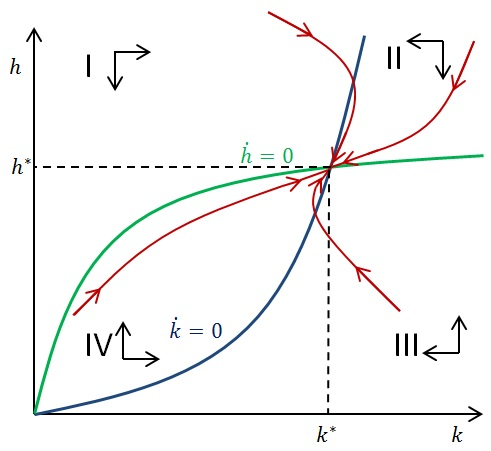
\includegraphics[scale=0.6]{plot_M-R-W}
	\caption{Фазовая диаграмма модели}
	\label{fig:plot_M-R-W}
\end{figure}

Устойчивое состояние модели можно выразить, подставляя полученные уравнения одно в другое:
\begin{ceqn}
	\begin{align*}
		k^* = \left(\dfrac{s_K^{1-\beta} \cdot s_H^\beta}{n + g + \delta}\right)^{\frac{1}{1-\alpha-\beta}}\\
		h^* = \left(\dfrac{s_K^{1-\alpha} \cdot s_H^\alpha}{n + g + \delta}\right)^{\frac{1}{1-\alpha-\beta}}
	\end{align*}
\end{ceqn}

\begin{ceqn}
	\begin{align*}
		y^* = \left(\dfrac{s_K^{\alpha} \cdot s_H^\beta}{(n + g + \delta)^{\alpha+\beta}}\right)^{\frac{1}{1-\alpha-\beta}}\\
	\end{align*}
\end{ceqn}

Линии $\dot{k} = 0$ -- синяя и $\dot{h} = 0$ -- зелёная делят диаграмму на четыре квадранта. Возможные траектории фондовооружённости показаны красным. В итоге, в модели из любой начальной точки система приходит к равновесию ($k^*, h^*$).

\subsubsection*{Численный анализ модели Солоу с человеческим капиталом}
\addcontentsline{toc}{subsubsection}{Численный анализ модели Солоу с человеческим капиталом}

\textbf{Задание:}\\
Провести численный анализ модели Солоу с человеческим капиталом.\\

\textbf{Решение:}\\
В соответствии с формулами, данная модель была реализована в среде моделирования AnyLogic. В качестве начальных параметров было принято решение взять $\alpha = 0.5$, $\beta = 0.2$, $s_K = 0.6$, $s_H = 0.9$, $\delta = 0.01$, $n = 0.3$, $g = 0.2$, $k_0 = 7$, $h_0 = 14$. (Рисунок \ref{fig:M-R-W_anylogic})
\begin{figure}[h]
	\centering 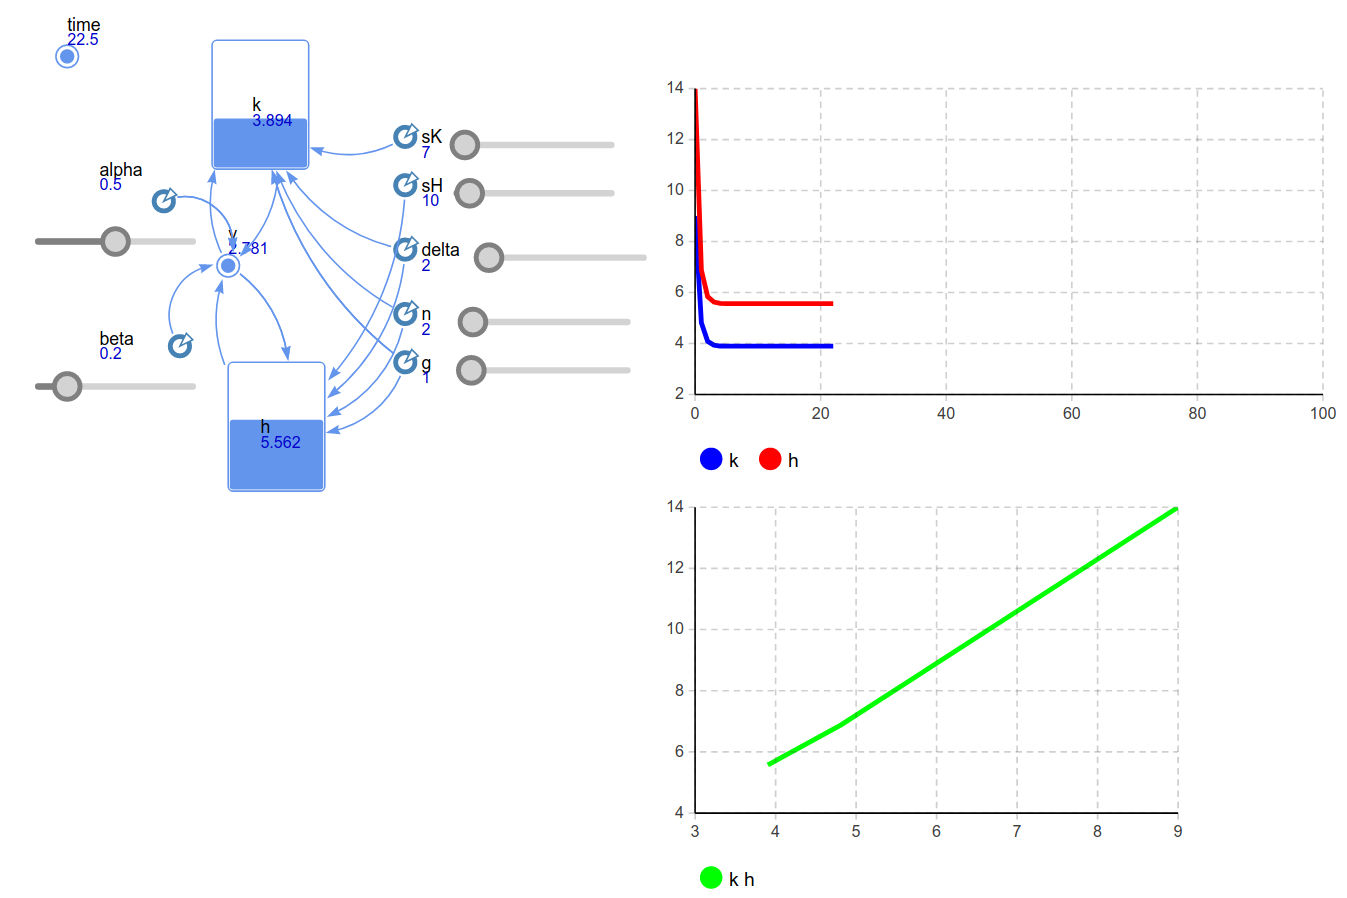
\includegraphics[scale=0.16]{M-R-W_anylogic}
	\caption{Результаты построения модели Солоу с человеческим капиталом в AnyLogic}
	\label{fig:M-R-W_anylogic}
\end{figure}

\newpage

Как можно заметить на графике, который демонстрирует изменение физического капитала и изменение человеческого капитала с течением времени, изначально имел место спад, а затем система пришла в стационарное состояние.\\

Также данная модель была реализована на языке программирования Python. Для решения системы дифференциальных уравнений был реализован и применён метод Рунге-Кутта. (Рисунок \ref{fig:M-R-W_runge_kutta})
\begin{figure}[h]
	\centering 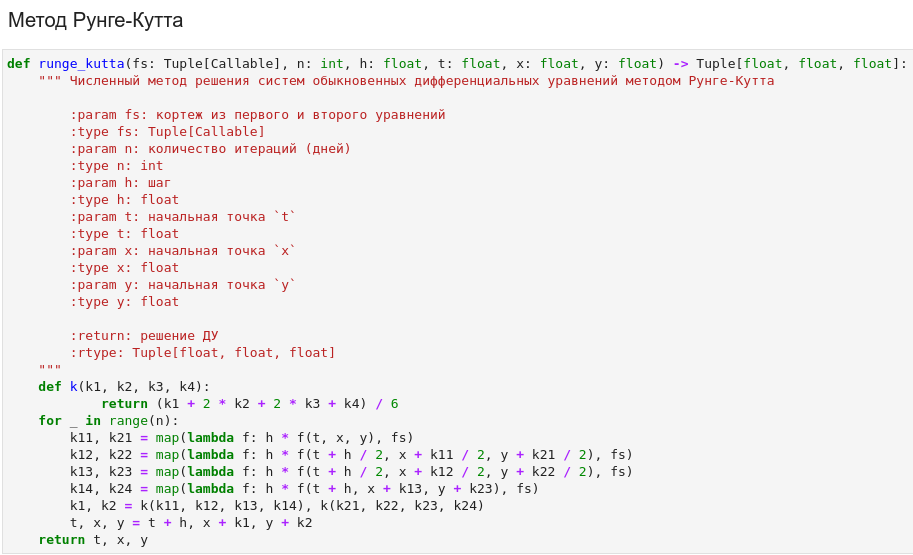
\includegraphics[scale=0.5]{M-R-W_runge_kutta}
	\caption{Метод Рунге-Кутта на языке программирования Python}
	\label{fig:M-R-W_runge_kutta}
\end{figure}

Параметры модели были взяты из AnyLogic. (Рисунок \ref{fig:M-R-W_python_result})
\begin{figure}[h]
	\centering 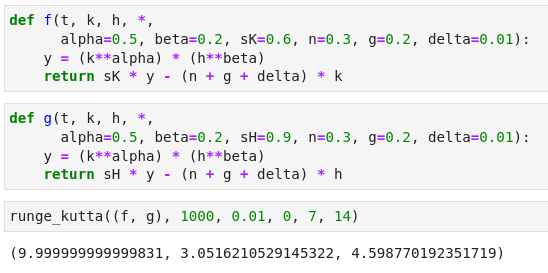
\includegraphics[scale=0.4]{M-R-W_python_result}
	\caption{Результаты построения модели Солоу с человеческим капиталом в Python для десятого момента времени}
	\label{fig:M-R-W_python_result}
\end{figure}

\newpage

На основании полученных результатов можно построить график, который демонстрирует изменение физического капитала ($k$) и изменение человеческого капитала ($h$) с течением времени. (Рисунок \ref{fig:M-R-W_python_result_plot})
\begin{figure}[h]
	\centering 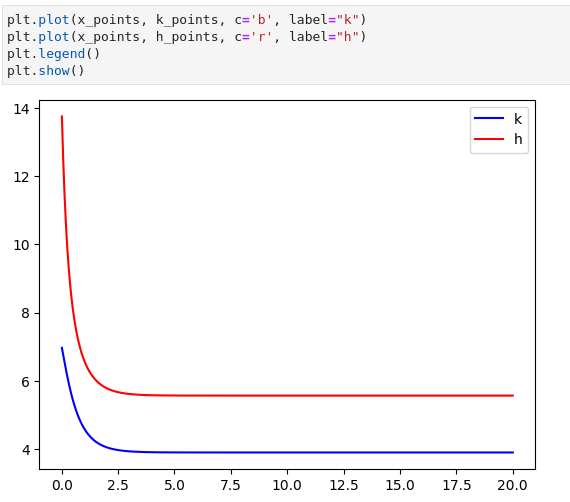
\includegraphics[scale=0.4]{M-R-W_python_result_plot}
	\caption{График изменение капиталов модели}
	\label{fig:M-R-W_python_result_plot}
\end{figure}

Как можно заметить данный график полностью соответствует графику, который был построен с помощью инструмента AnyLogic.\\

Также если изменять параметры модели, то она всё равно будет приходить в устойчивое состояние. (Рисунок \ref{fig:M-R-W_anylogic_variance})
\begin{figure}[h]
	\centering 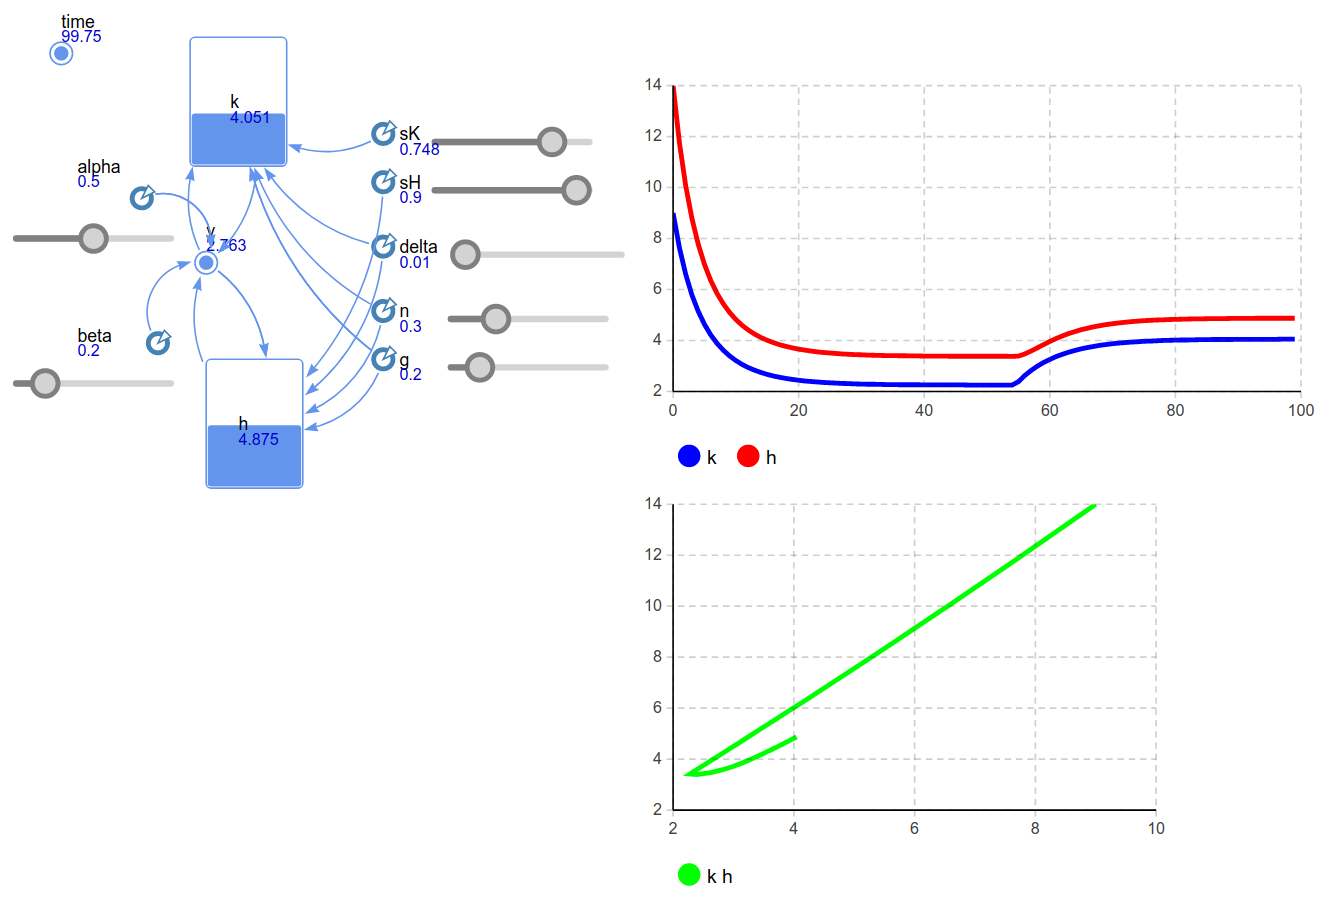
\includegraphics[scale=0.25]{M-R-W_anylogic_variance}
	\caption{Изменение параметров модели}
	\label{fig:M-R-W_anylogic_variance}
\end{figure}